\documentclass[discrete.tex]{subfiles}

\begin{document}
  \section{Основные определения теории графов}

  \begin{definition}
    Граф $G = <M, N, T>$, где M,N - конечные мн-ва,
    \[T: N \ra M \times M\]
    M - мн-во вершин, N - мн-во дуг/ребер
  \end{definition}

  Способы задания графа:
  \begin{enumerate}
    \item Схема (на ней просто нумерация)
    \begin{figure}[H]
            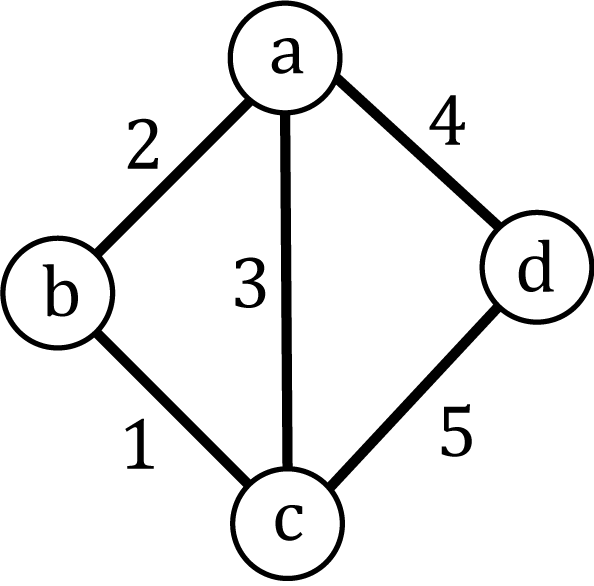
\includegraphics[width=3cm]{pics/36_1}
            \centering
    \end{figure}
    \item T-список:\\
    1-(a,c)\\
    2-(a,b)\\
    3-(c,b)\\
    4-(b,d)\\
    5-(c,d)
    \item Матрица смежности $r[M,M]$
    \[r[i,j]=1,\qq \e(i,j)\]
    \[r[i,j]=0,\qq \text{нет}\]
    \begin{tabular}{c|c|c|c|c}
      \ & a & b & c & d\\
      \hline
      a & 0 & 1 & 1 & 0\\
      \hline
      b & 1 & 0 & 1 & 1\\
      \hline
      c & 1 & 1 & 0 & 1\\
      \hline
      d & 0 & 1 & 1 & 0
    \end{tabular}
    \item Матрица инденденций $a[M,N]$ (то есть что из вершин выходит)
    \begin{tabular}{c|c|c|c|c|c}
      \ & 1 & 2 & 3 & 4 & 5\\
      \hline
      a & 1 & 1 & 0 & 0 & 0\\
      \hline
      b & 0 & 1 & 1 & 1 & 0\\
      \hline
      c & 1 & 0 & 1 & 0 & 1\\
      \hline
      d & 0 & 0 & 0 & 1 & 1
    \end{tabular}
    (если граф направленный, то ставить $\pm 1$)
  \end{enumerate}

  \begin{definition}[по Григорьевой]
    \begin{enumerate}
      \item Цепью звенности k называется последовтельность $i_1 u_1 i_2 u_2 i_3 ... u_{k-1} i_k$
      \[u_t = (i_t, i_{t+1}), \q \forall t \in 1,...,k-1\]
      \item Путём то же самое, но $u_t = i_t \ra i_{t+1}$
      \item Дуга, выходящая из вершины и входящая в неё же называется петлёй $u_i=(i_i,i_i)$
      \item Цикл - путь, у которой $i_1 = i_k$
      \item Контур - путь, у которого $i_1 = i_k$
      \item $G'=<M',N'>$ - частичный граф $<M,N>$, если $M' \subset M$, $N' \subset N$
    \end{enumerate}
  \end{definition}

  \begin{definition}[по Романовскому]
    \begin{enumerate}
      \item Путем звенности k в графе $<M,N,T>$ называется пара отображений A: $1:k \ra N$, V: $0:k \ra M$, таких что $\forall i \in 1:k$ выполняется: $\End A(i)=V(i)$ и $\Beg A(i) = V(i-1)$
      \item Тройка $<M, N', T>$, где $N' \subset N$ называется частичным графом графа $<M,N,T>$ (строго говоря тут $T'$, ограничение на отображение $T$)
      \item Пусть $M' \subset M$, обозначим через $N(M')$ мн-во всех дуг, у которых начала и концы принадлежат $M'$
      \item Граф $<M', N', T>$ называется подграфом графа $<M,N,T>$. Граф $<M',N',T>$, где $N' \subset N(M')$ называется частичным подграфом графа $<M,N,T>$
      \item Частичный подграф $<M',N',T>$ называется простным путем, если:
      \begin{enumerate}
        \item Число его дук $k$ на единицу меньше числа вершин
        \item Можно так перенумеровать $M'$ числами от $0$ до $k$ и $N'$ числами от $1$ до $k$, что для любой другой дуги $u \in N'$
        \[\num(u) = \num (\End u) = \num(\Beg u) + 1\]

        То есть в определениях Григорьевой без второго условия это путь, а со всеми - это путь, у которого каждая дуга втречается не более одного раза
      \end{enumerate}
      \begin{figure}[H]
              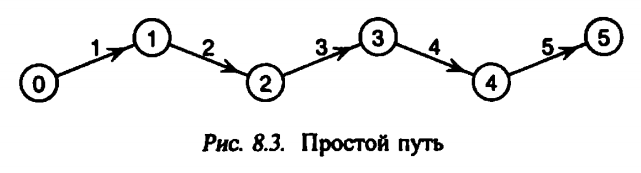
\includegraphics[width=5cm]{pics/36_2}
              \centering
      \end{figure}
      \item Отношение транзитивно, если для любого пути в графе, соответствующему этому отношению, найдется дуга, идущая из начала пути в его конец (т.е. если любой путь "дублируется"{} соответствующий в графе дугой)
      \item Частичный подграф $<M',N',T>$ называется цепью, если:
      \begin{enumerate}
        \item Число дуг $k$ на единицу меньше числа вершин
        \item Можно так перенумеровать $M'$ числами от $0$ до $k$ и $N'$ числами от $1$ до $k$, что для любой дуги $u \in N'$
        \[\num(u) = \num(\End u) = \num(\Beg u) + 1\]
        либо
        \[\num(u) = \num(\End u) + 1 = \num(\Beg u)\]
      \end{enumerate}
      \begin{figure}[H]
              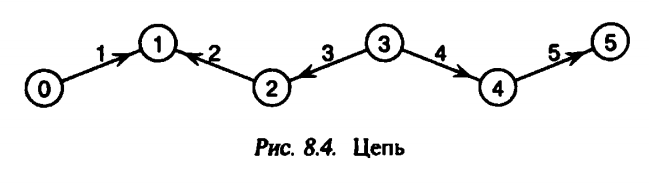
\includegraphics[width=5cm]{pics/36_3}
              \centering
      \end{figure}
      \item Дуги деляется на положительно ориентированные и отрицательно ориентированные
      \item Частичный подграф $<M',N',T>$ называется контуром, если:
      \begin{enumerate}
        \item Число дуг $k$ равно числу вершин
        \item Можно так перенумеровать $M'$ и $N'$ числами от $1$ до $k$, что для любой дуги $u \in N'$
        \[\num(u) \os{\mod k}{=} \num(\End u) \os{\mod k}{=} \num(\Beg u) + 1\]
      \end{enumerate}
      Т.е. контур - это простой путь, в котором начало и конец совпадают
      \begin{figure}[H]
              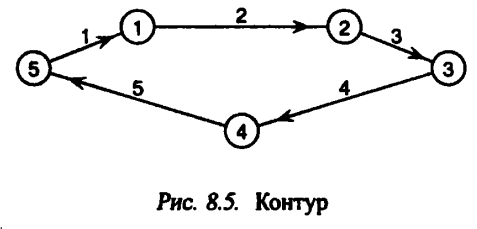
\includegraphics[width=5cm]{pics/36_4}
              \centering
      \end{figure}
      \item Частичный подграф $<M',N',T>$ называется циклом, если:
      \begin{enumerate}
        \item Число дуг k равно числу вершин
        \item Можно так перенумеровать $M'$ и $N'$ числами от 1 дл k, что для любой дуги $u \in N'$
        \[\num(u) \os{\mod k}{=} \num(\End u) \os{\mod k}{=} \num(\Beg u) + 1\]
        либо
        \[\num(u) \os{\mod k}{=} \num(\End u) + 1 \os{\mod k}{=} \num(\Beg u)\]
      \end{enumerate}
      Т.е. цикл - это цепь, в которой начало и конец совпадают
    \end{enumerate}
    \begin{figure}[H]
            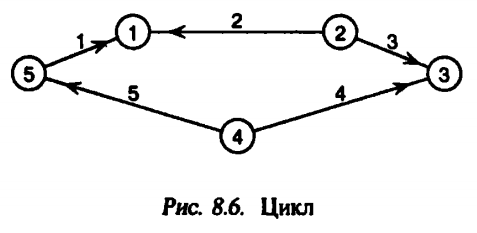
\includegraphics[width=5cm]{pics/36_5}
            \centering
    \end{figure}
  \end{definition}

  \begin{definition}
    Граф называется связным, если любые его две вершины соеденены цепью
  \end{definition}

  \begin{definition}
    Граф называется ациклическим, если в нем нет циклов
  \end{definition}

  \begin{ttheorem}[с.218]

  \end{ttheorem}
\end{document}
